% DFA for an LR parser
\documentclass{article}
\usepackage{tikz}
\usetikzlibrary{arrows.meta,decorations.pathmorphing,backgrounds,positioning,fit,petri}
\begin{document}
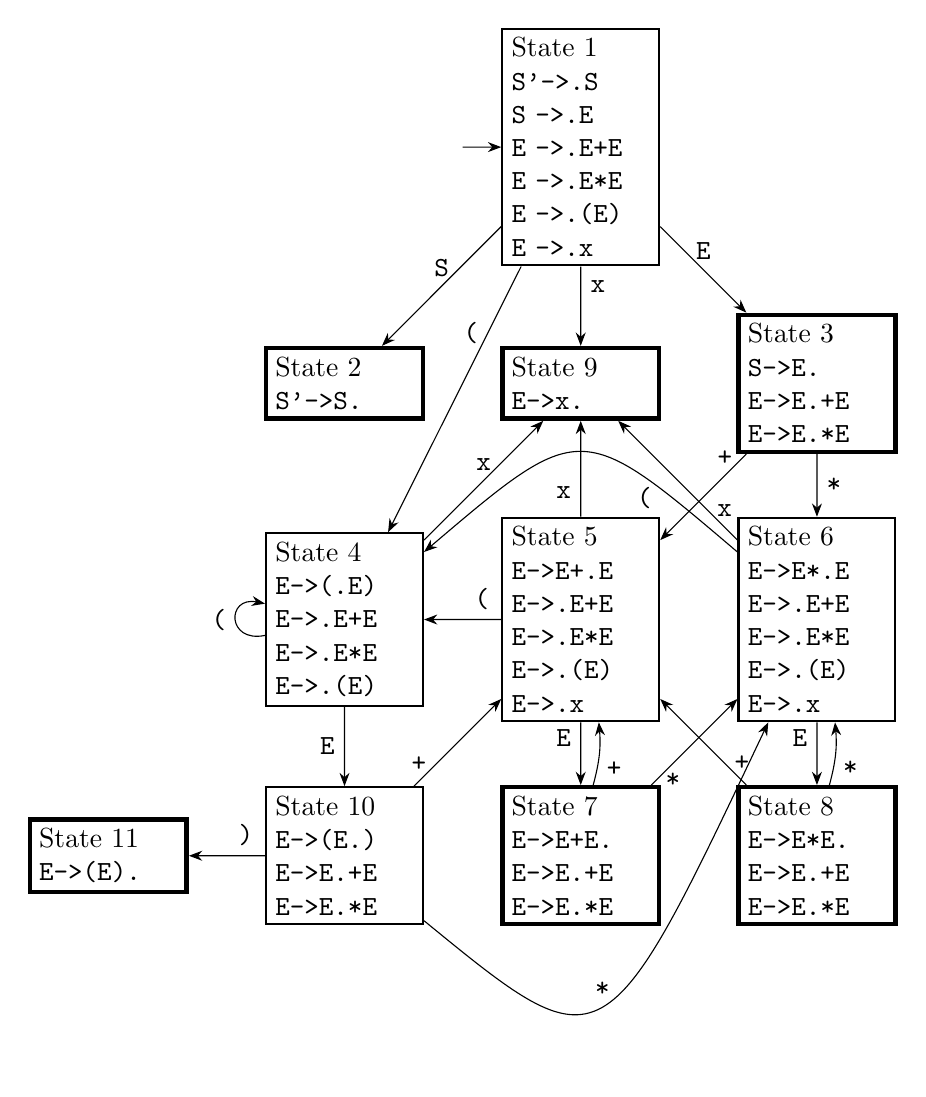
\begin{tikzpicture}[scale=3, >=Stealth,
   state/.style={rectangle, text width=50, thick},
   final/.style={ultra thick}]
   \node (q1) at (2,7) [draw, state] {State 1\\
\texttt{S'->.S}\\
\texttt{S ->.E}\\
\texttt{E ->.E+E}\\
\texttt{E ->.E*E}\\
\texttt{E ->.(E)}\\
\texttt{E ->.x}};
   \node (q2) at (1, 6) [draw, state, final] {State 2\\
\texttt{S'->S.}};
   \node (q3) at (3, 6) [draw, state, final] {State 3\\
\texttt{S->E.}\\
\texttt{E->E.+E}\\
\texttt{E->E.*E}};
   \node (q4) at (1, 5) [draw, state] {State 4\\
\texttt{E->(.E)}\\
\texttt{E->.E+E}\\
\texttt{E->.E*E}\\
\texttt{E->.(E)}};
   \node (q5) at (2, 5) [draw, state] {State 5\\
\texttt{E->E+.E}\\
\texttt{E->.E+E}\\
\texttt{E->.E*E}\\
\texttt{E->.(E)}\\
\texttt{E->.x}};
   \node (q6) at (3, 5) [draw, state] {State 6\\
\texttt{E->E*.E}\\
\texttt{E->.E+E}\\
\texttt{E->.E*E}\\
\texttt{E->.(E)}\\
\texttt{E->.x}};
   \node (q7) at (2, 4) [draw, state, final] {State 7\\
\texttt{E->E+E.}\\
\texttt{E->E.+E}\\
\texttt{E->E.*E}};
   \node (q8) at (3, 4) [draw, state, final] {State 8\\
\texttt{E->E*E.}\\
\texttt{E->E.+E}\\
\texttt{E->E.*E}};
   \node (q9) at (2, 6) [draw, state, final] {State 9\\
\texttt{E->x.}};
   \node (q10) at (1, 4) [draw, state] {State 10\\
\texttt{E->(E.)}\\
\texttt{E->E.+E}\\
\texttt{E->E.*E}};
   \node (q11) at (0, 4) [draw, state, final] {State 11\\
\texttt{E->(E).}};

   \draw (q1)[<-] -- ++(-0.5,0);
   \draw (q1)[->] -- node[above]{\texttt{S}} (q2);
   \draw (q1)[->] -- node[above]{\texttt{E}} (q3);
   \draw (q1)[->] -- node[left, near start]{\texttt{(}} (q4);
   \draw (q1)[->] -- node[right, near start]{\texttt{x}} (q9);

   \draw (q3)[->] -- node[above, near start]{\texttt{+}} (q5);
   \draw (q3)[->] -- node[right]{\texttt{*}} (q6);

   \draw (q4)[->] .. controls ++(-0.5, -0.1) and ++(-0.5,0.1) .. node[left]{\texttt{(}} (q4);
   \draw (q4)[->] -- node[above]{\texttt{x}} (q9);
   \draw (q4)[->] -- node[left]{\texttt{E}} (q10);

   \draw (q5)[->] -- node[above, near start]{\texttt{(}} (q4);
   \draw (q5)[->] -- node[left, near start]{\texttt{E}} (q7);
   \draw (q5)[->] -- node[left, near start]{\texttt{x}} (q9);

   \draw (q6)[->] .. controls ++(-1, 0.85) .. node[below, near start]{\texttt{(}} (q4);
   \draw (q6)[->] -- node[left, near start]{\texttt{E}} (q8);
   \draw (q6)[->] -- node[right, near start]{\texttt{x}} (q9);

   \draw [->] (q7) to [bend right=10] node[right, near start]{\texttt{+}} (q5);
   \draw (q7)[->] -- node[below, near start]{\texttt{*}} (q6);

   \draw (q8)[->] -- node[right, near start]{\texttt{+}} (q5);
   \draw (q8)[->] to [bend right=10] node[right, near start]{\texttt{*}} (q6);

   \draw (q10)[->] -- node[left, near start]{\texttt{+}} (q5);
   \draw (q10)[->] .. controls ++(1.1, -0.9) .. node[above]{\texttt{*}} (q6);
   \draw (q10)[->] -- node[above, near start]{\texttt{)}} (q11);

\end{tikzpicture}
\end{document}
